%! Author = Pascal Bakker
%! Date = 04/05/2024

%-------------------------------------------------------------------------------
% TEMPLATE
%-------------------------------------------------------------------------------
\documentclass[balance=false,nonacm,sigconf]{acmart}

\settopmatter{printacmref=false} % Removes citation information below abstract
\renewcommand\footnotetextcopyrightpermission[1]{} % removes footnote with conference information in first column

\AtBeginDocument{%
    \providecommand\BibTeX{{%
        \normalfont B\kern-0.5em{\scshape i\kern-0.25em b}\kern-0.8em\TeX}}}

% support special characters
\usepackage[T1]{fontenc}
\usepackage{lmodern}

%-------------------------------------------------------------------------------
% PACKAGES FOR URL
%-------------------------------------------------------------------------------
\hypersetup{colorlinks, citecolor=blue, filecolor=blue, linkcolor=blue, urlcolor=blue}
\usepackage{xurl}

%-------------------------------------------------------------------------------
% PACKAGES AND COMMANDS FOR TABLES
%-------------------------------------------------------------------------------
\usepackage{longtable}
\usepackage{multirow}
\usepackage{adjustbox}
\usepackage{color,colortbl,xcolor}
\usepackage{array}
\newcolumntype{L}[1]{>{\raggedright\renewcommand{\newline}{\\}\arraybackslash\hspace{0pt}}m{#1}}
\newcolumntype{C}[1]{>{\centering\renewcommand{\newline}{\\}\arraybackslash\hspace{0pt}}m{#1}}
\newcolumntype{R}[1]{>{\raggedleft\renewcommand{\newline}{\\}\arraybackslash\hspace{0pt}}m{#1}}

%-------------------------------------------------------------------------------
% PACKAGES FOR FIGURES
%-------------------------------------------------------------------------------
\usepackage{graphicx,graphics,float,subfigure,wrapfig,epstopdf}
\usepackage{dblfloatfix} %to fix the problem of [h!] [t!] [!b]
\epstopdfsetup{update}

%-------------------------------------------------------------------------------
% PACKEGE FOR CREATING GANTT VISUALIZATION (PLANNING TABLE)
%-------------------------------------------------------------------------------
\usepackage{soul}
\usepackage{pgfgantt} %for the planning table

%-------------------------------------------------------------------------------
% CREATING COMMANDS FOR AUTOREF
%-------------------------------------------------------------------------------
\renewcommand{\chapterautorefname}{\S}
\renewcommand{\sectionautorefname}{\S}
\renewcommand{\subsectionautorefname}{\S}
\renewcommand{\subsubsectionautorefname}{\S}
\newcommand{\subfigureautorefname}{\figureautorefname}

%-------------------------------------------------------------------------------
% COPYRIGHT
%-------------------------------------------------------------------------------
\setcopyright{acmcopyright}
\copyrightyear{2024}
\acmYear{2024}

%-------------------------------------------------------------------------------
% BEGIN DOCUMENT
%-------------------------------------------------------------------------------
\begin{document}

%-------------------------------------------------------------------------------
% TITLE
%-------------------------------------------------------------------------------
    \title[Automating the Cybersecurity Triage Process]{Automating the Cybersecurity Triage Process: A Comparative Study on the Performance of Large Language Models}

%-------------------------------------------------------------------------------
% AUTHORS
%-------------------------------------------------------------------------------
    \author{Pascal Bakker}
    \email{p.n.bakker@student.utwente.nl}
    \affiliation{%
        \institution{University of Twente}
        \streetaddress{P.O. Box 217}
        \city{Enschede}
        \country{The Netherlands}
        \postcode{7500AE}
    }

%-------------------------------------------------------------------------------
% ABSTRACT AND KEYWORDS
%-------------------------------------------------------------------------------
    % context
% problem
% difference from literature
% proposal
% expected contributions
\begin{abstract}
    In Security Information and Event Management, alarms are created when certain conditions are met.
    Security analysts have the task to inspect alarms to filter false positives and identify their severity: triage.
    This process is complicated and time-consuming, limiting the depth and speed of investigations.
    Whereas other proposed optimizations and automations appear to be very promising, rapid advancements in Natural Language Processing and the development of Large Language Models (LLMs) opened up new possibilities to speed up the triage process.
    This research will identify ways in which LLMs can optimize triage, evaluate the performance of these techniques and offer a comparison between different LLMs.
    The results of this research are expected to help security teams in making informed implementation decisions when optimizing the triage process.
\end{abstract}
    \keywords{Cybersecurity, llm, triage}

%-------------------------------------------------------------------------------
%-------------------------------------------------------------------------------
    \maketitle

%-------------------------------------------------------------------------------
% SECTIONS
%-------------------------------------------------------------------------------
    \section{Introduction} 
\label{sec:introduction}


\comment{The Introduction section has more or less the same structure as your abstract. The difference is that in the abstract each part is one statement/phrase, while in the introduction each part is a paragraph. So, (i) context, (ii) problem, (iii) proposal, and your most astonishing (iv) finding. Of course in the Introduction section you can give far more details than in the abstract. Avoid to copy and paste statements, re-write with different words.}

\comment{In addition to the structure that you already know you should include your \textit{research questions} between the ``proposal'' paragraph and the ``findings''. The statement that precede the RQ is something like the following: }

To pursue our goal, we have defined the following research questions (RQ) as the basis of our research: 
\begin{itemize}	
	\item \textbf{RQ1:} What are ..?
	\item \textbf{RQ2:} How to ... ?
	 \item \textbf{RQ3:} How to ...?
\end{itemize}



\comment{Please, avoid "yes or no" questions. Make questions that your reader are not able to answer immediately. Usually the questions depend on each other, it means that to answer one question you must answer the one before.}

\comment{Before a little bit of your most astonishing findings you must to introduce the structure of your paper (or proposal). Usually the text looks like the following.}
 
``The remainder of this paper (or proposal) is organized as follows. Section 2 will discuss the approaches expected for answering each research question. After that, we present a preliminary planning for the research questions in Section 3. Finally, we conclude with a proposal and planning for the thesis structure in Section 4.'' 






    \section{Related Work}
\label{sec:related-work}

*Check connectedpapers.com

\begin{enumerate}
    \item A Survey of Large Language Models in Cybersecurity
    \item Review of Generative AI Methods in Cybersecurity
    \item
\end{enumerate}

For the phase after the proposal you should re-read those interesting papers and take note of their "related work" papers. Read those papers and update the Excel Sheet.

\textbf{NOTE: that the final goal of this section is a table that summarizes the characteristics of each paper and your critical analysis to highlight the existing gaps of research.}

Examples of how to make a reference:
\begin{itemize}
    \item $\backslash$citep outputs:~\citep{jjsantanna2015IM1}
    \item $\backslash$citet outputs: \citet{jjsantanna2015IM1}
\end{itemize}

    \section{Methodologies}
<brief summary explaining the content and the connection><you could even to make a picture explaining how the parts connect for example a conceptual figure with your idea (if possible). On this, I must say that Figures MUST be in pdf format (I like to use Inkscape to create my figures, then I export to pdf) [ask me how, for help]> 

\subsection{On answering RQ1}

\subsection{On answering RQ2}

\subsection{On answering RQ3}
\begin{figure}[h!]
	\label{fig:approach}
	\centering
	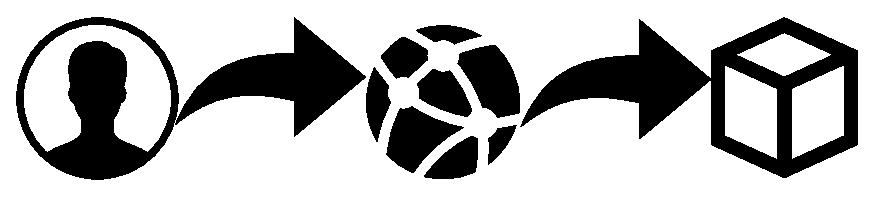
\includegraphics[width=0.45\textwidth]{figs/example.eps}
	\caption{Example of Figure.}
\end{figure}
    \section{Planning}
 In this section we will shortly discuss the planning of the study. The study has been split into six parts, as can be seen in the table below. Note that a planning such as this when is to be seen as a guideline. There are however some hard deadlines for handing in drafts and final versions. Here we have an overview of the deadlines:
 \begin{itemize}	
	\item December 1st: Final proposal submission
	\item January 19th: Draft paper submission
	\item January 26th: Final paper submission
	\item January 31th: Conference presentation
\end{itemize}
The planning is made in order to adhere to these submission deadlines.

% More examples on how to do a planning table you can see in \url{http://www.martin-kumm.de/wiki/doku.php?id=05Misc:A_LaTeX_package_for_gantt_plots}

\begin{figure}[ht]
		\noindent\resizebox{0.49\textwidth}{!}{
	\begin{gantt}[xunitlength=0.5cm,fontsize=\small,titlefontsize=\small,drawledgerline=true]{15}{12} %(1)lines (2)columns
		
		\begin{ganttitle} %Month
			\titleelement{\textbf{Planning Table}}{12}
		\end{ganttitle}
		
		\begin{ganttitle} %Month
			\titleelement{November}{3}
			\titleelement{December}{5}
			\titleelement{January}{4}
		\end{ganttitle}
		\begin{ganttitle} % Week number
			\numtitle{1}{1}{12}{1}
		\end{ganttitle}
		\ganttbar[color=gray]{Proposal}{0}{3}
		\ganttmilestone[color=orange]{Draft proposal}{2}
		\ganttmilestone[color=red]{Final proposal}{3}
		\ganttbar[pattern=grid,color=orange]{Writing}{3}{8}
		\ganttbar[color=blue]{RQ1}{3}{1}
		\ganttcon{3}{3}{3}{7}
		\ganttbarcon[color=blue]{RQ2}{4}{2}
		\ganttbar[pattern=grid,color=red]{Holidays}{6}{2}
		\ganttbar[color=blue]{RQ3}{8}{2}
		\ganttcon{6}{8}{8}{10}
		\ganttbarcon[color=blue]{RQ4}{10}{1}
		\ganttmilestone[color=orange]{Draft Paper submission}{10}
		\ganttmilestone[color=red]{Final Paper submission}{11}
		\ganttbar[color=green]{Presentation}{11}{1}
		\ganttcon{11}{11}{11}{14}

	\end{gantt}	
		}
\end{figure}



% The research topics part consists solely of a literature study that focuses on ... All relevant information learned from this will be integrated in a survey that will form the first part of the thesis.

% Following the research topics are each of the research questions, with time allotted at the end of each research question to integrate the results into the thesis. 

%-------------------------------------------------------------------------------
% REFERENCES
%-------------------------------------------------------------------------------
    \bibliographystyle{ACM-Reference-Format}
    \bibliography{bibliography}

%-------------------------------------------------------------------------------
% END DOCUMENT
%-------------------------------------------------------------------------------
\end{document}
\endinput
